% !TeX encoding = UTF-8
% !TeX spellcheck = en_US
% !TeX TS-program = lualatex
% !TEX root = exampleGR.tex
\documentclass{GR}
\addbibresource{exampleGR.bib}

% FONTS NOTE: This example uses fonts similar to those used by Genome Research,
% but you may have different fonts installed in your system. If you compile the
% doc and run into trouble with the fonts, just open the GR.cls file and change
% the fonts to your preferred ones.

% BIB NOTE: This example uses BibLaTeX with biber as backend.

% release codenumber (update it here!)


%%% DOCUMENT %%%

\begin{document}

%===================================== 1. AUTHOR AND TITLE PAGE =======================================

\title{
	\vspace*{0mm} % May help to include the corresponding author footnote in the title page
	%\singlespacing
    \doublespacing
	% \begin{flushleft}
	% 	\texttt{\large Title:} \\
	% \end{flushleft}
	\vspace*{2mm}
    
	{\Huge\titlefont scHiC-Mamba: this is a example title}\\
	\vspace*{4mm}
    % \begin{flushleft}
    %     \texttt{\large Running Title:} \\
    % \end{flushleft}
    % \vspace*{0mm}
    % % {\Huge\rtitlefont scHiC-Diff}
    % \vspace*{4mm}
    
	}

\doublespacing
% ===== Authors =====
\author[1,\#]{\mdseries\Large\authorfont XX Du}
\author[1,\#]{\mdseries\Large\authorfont ZZ Fang}
\author[1,\#]{\mdseries\Large\authorfont WW Liu}
\author[2]{\mdseries\Large\authorfont LL Tang}
\author[1,*]{\mdseries\Large\authorfont MM Li}

% ===== Footnotes (equal contribution + corresponding author) =====
% \begin{NoHyper}
% \relax\renewcommand\thefootnote{\#}\footnotetext{These authors contributed equally to this work.}
% \relax\renewcommand\thefootnote{*}\footnotetext{Correspondence: ****@mail.***.edu.cn}
% \end{NoHyper}

% ===== Affiliations =====
\affil[1]{\sffamily\slshape\large School of Computer Science and Engineering, Central South University, Changsha, Hunan 410083, P.R. China.}
\affil[2]{\sffamily\slshape\large Department of Genetics, ******, *****, ****, USA.}

% \date{}
% % \date{January 19, 2026}


\maketitle

\begin{flushleft}
{\sffamily\slshape\large
{\#}These authors contributed equally to this work. \\
{*}Correspondence: \href{mailto:example@mail.csu.edu.cn}{example@mail.csu.edu.cn}
}
\vspace*{3mm}
\end{flushleft}


\begin{flushleft}
    {\sffamily\slshape\large\textbf{Running title:}  scHiC-Mamba} \\
\vspace*{0mm}
% {\sffamily\slshape\large scHiC-Diff}
\end{flushleft}
% \vspace*{4mm}

\clearpage


%===================================== 2. ABSTRACT PAGE=======================================
%%% Abstract

{\abstract{Single-cell high-throughput chromosome conformation capture (scHi-C) enables the analysis of cell-to-cell variability in three-dimensional (3D) genome organization.} 

\begin{keywords}
	single-cell Hi-C, cell clustering
\end{keywords}

\clearpage


%===================================== 3. SECTIONS ===========================================
%%% Introduction

\section*{Introduction}

Three-dimensional (3D) genome organization plays a critical role in gene regulation, Three-dimensional (3D) genome organization plays a critical role in gene regulation, DNA replication, and overall cellular function. Three-dimensional (3D) genome organization plays a critical role in gene regulatio, Three-dimensional (3D) genome organization plays a critical role in gene regulatio, Three-dimensional (3D) genome organization plays a critical role in gene regulatio.

Three-dimensional (3D) genome organization plays a critical role in gene regulation, Three-dimensional (3D) genome organization plays a critical role in gene regulation, DNA replication, and overall cellular function. Three-dimensional (3D) genome organization plays a critical role in gene regulatio, Three-dimensional (3D) genome organization plays a critical role in gene regulatio, Three-dimensional (3D) genome organization plays a critical role in gene regulatio.

Three-dimensional (3D) genome organization plays a critical role in gene regulation, Three-dimensional (3D) genome organization plays a critical role in gene regulation, DNA replication, and overall cellular function. Three-dimensional (3D) genome organization plays a critical role in gene regulatio, Three-dimensional (3D) genome organization plays a critical role in gene regulatio, Three-dimensional (3D) genome organization plays a critical role in gene regulatio.

%%% Results
\section*{Results}
\subsection*{Overview of scHiC-Mamba}
Three-dimensional (3D) genome organization plays a critical role in gene regulation, Three-dimensional (3D) genome organization plays a critical role in gene regulation, DNA replication, and overall cellular function. Three-dimensional (3D) genome organization plays a critical role in gene regulatio, Three-dimensional (3D) genome organization plays a critical role in gene regulatio, Three-dimensional (3D) genome organization plays a critical role in gene regulatio.

Three-dimensional (3D) genome organization plays a critical role in gene regulation, Three-dimensional (3D) genome organization plays a critical role in gene regulation, DNA replication, and overall cellular function. Three-dimensional (3D) genome organization plays a critical role in gene regulatio, Three-dimensional (3D) genome organization plays a critical role in gene regulatio, Three-dimensional (3D) genome organization plays a critical role in gene regulatio (Figure~\ref{fig:model}). 


	
\begin{figure*}[tbp]
    \centering
    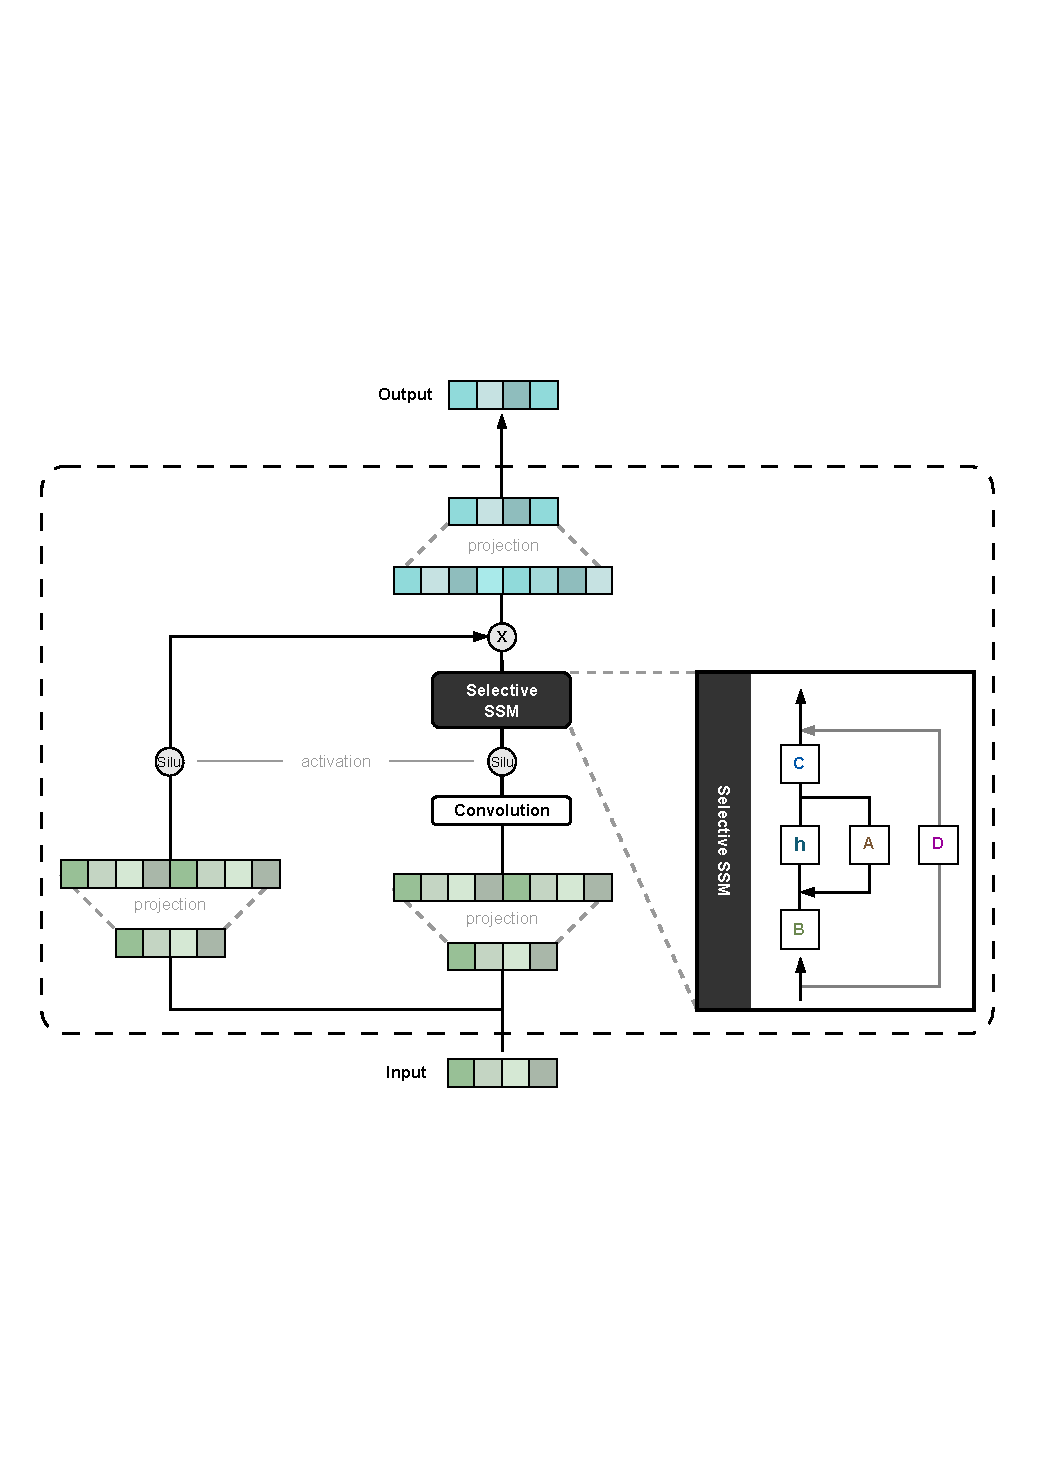
\includegraphics[width=0.99\textwidth]{./figs/fig011.pdf}  
    \caption{
        \textbf{example: Framework of scHiC-Mamba.} In each training iteration, the scHi-C data $\boldsymbol{x}_0 $ is added with a corresponding noise disturbance.
    } 
    \label{fig:model}
\end{figure*}




\subsection*{effectively improves data quality}

We evaluate the uster~\parencite{zhou2019robust}, HiCImpute~\parencite{xie2022hicimpute}, scVI-3D~\parencite{zheng2022normalization} , and Higashi~\parencite{zhang2022multiscale}. The simulated datasets are adopted from HiCImpute~\parencite{xie2022hicimpute} and comprise three cell types evaluated at three sequencing depths (Supplementary TABLE S1).

Three-dimensional (3D) genome organization plays a critical role in gene regulation, Three-dimensional (3D) genome organization plays a critical role in gene regulation, DNA replication, and overall cellular function. Three-dimensional (3D) genome organization plays a critical role in gene regulatio, Three-dimensional (3D) genome organization plays a critical role in gene regulatio, Three-dimensional (3D) genome organization plays a critical role in gene regulatio.


\section*{Discussion}

Discussion Discussion Discussion. Discussion Discussion Discussion. Discussion Discussion Discussion.   

%%% Methods

\section*{Methods}
\subsection*{Datasets}

Datasets Datasets Datasets. Datasets Datasets Datasets. Datasets Datasets Datasets.

\subsection*{Training process}

Training process Training process Training process. Training process Training process Training process. Training process Training process Training process.


\subsection*{Sampling process}

Sampling process Sampling process Sampling process. Sampling process Sampling process Sampling process. Sampling process Sampling process Sampling process.·


\subsection*{Details of network}

Details of network Details of network Details of network. Details of network Details of network Details of network. Details of network Details of network Details of network.

\subsection*{Baselines}

Baselines Baselines Baselines. Baselines Baselines Baselines. Baselines Baselines Baselines.

\subsection*{Evaluation metrics}
Evaluation metrics Evaluation metrics Evaluation metrics. Evaluation metrics



\section*{Software availability}
The source code of scHiC-Mamba is publicly available at \href{https://github.com/********}{https://github.com/********}.



\section*{Competing interest statement}
The authors declare no competing interests.



\section*{Acknowledgment}
We are grateful to the High-Performance Computing Center of Central South University for partial support of this work. 

\textit{Funding:} This work was supported by the National Natural Science Foundation of China under Grant No.********.

\textit{Author contributions:}
X.D., Z.F., and W.L. contributed equally to this work.
X.D., Z.F., and W.L. designed the study.
X.D. implemented the proposed model.
X.D. and W.L. conducted the experiments.
X.D., Z.F., and W.L. wrote the manuscript.
T.L. assisted in data processing and analysis.
M.L. supervised the project and critically revised the manuscript.
All authors read and approved the final manuscript.














%===================================== BIBLIOGRAPHY =======================================
\printbibliography

\end{document}
